\subsection*{Task 2}

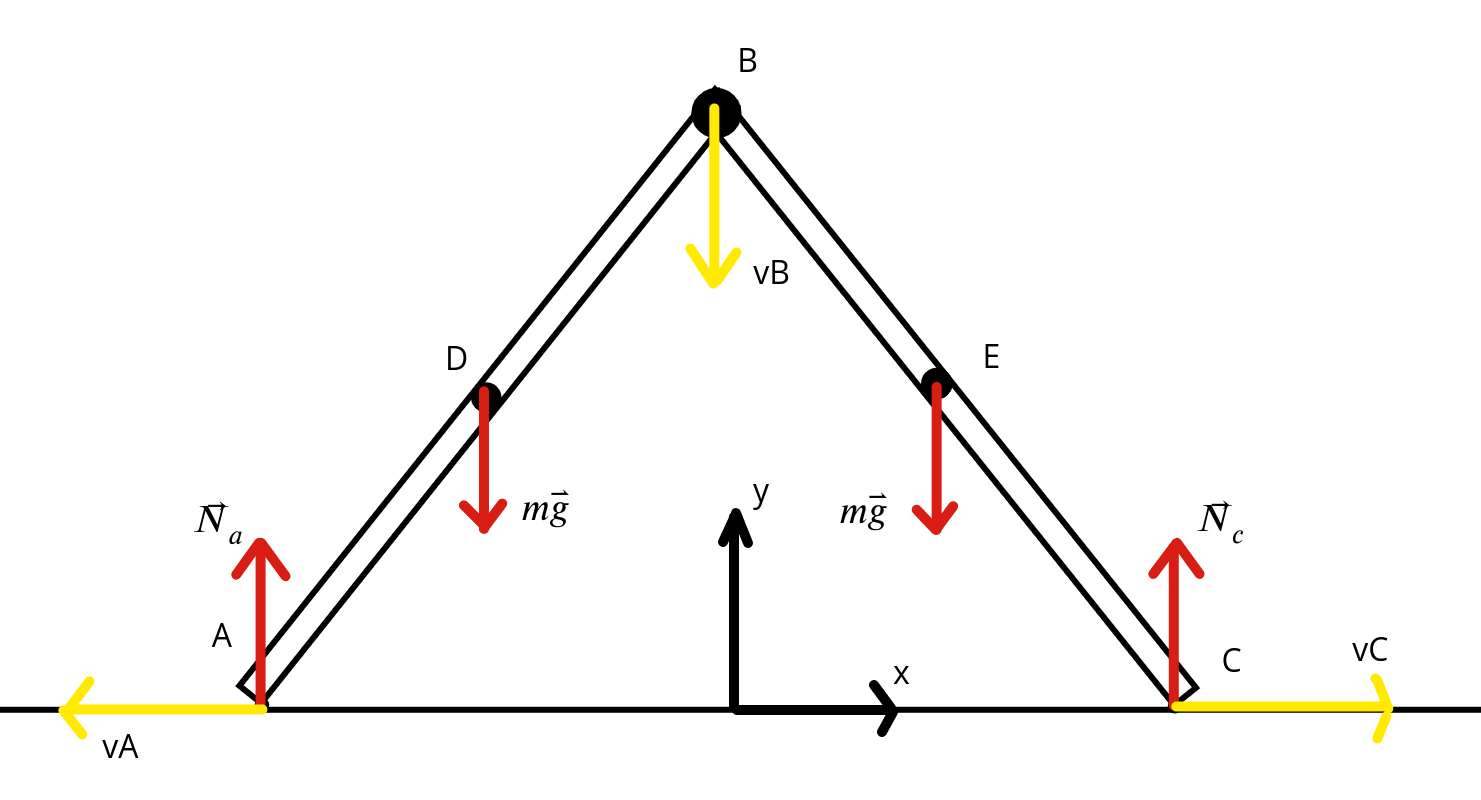
\includegraphics[width=\linewidth]{task2init.png}

\begin{enumerate}
    \item RO: system of 2 rods AB, BC
    \item Method: Theorem of change of kinetic energy (correlation between displacement and velocity)
    \item Force analysis:
          \[\vec{N}_a, \vec{N}_c, m_{AB}\vec{g}, m_{BC}\vec{g} \] \\
          There are no forces along x-axis $\implies$ B will hold its x position
    \item Conditions: \\
          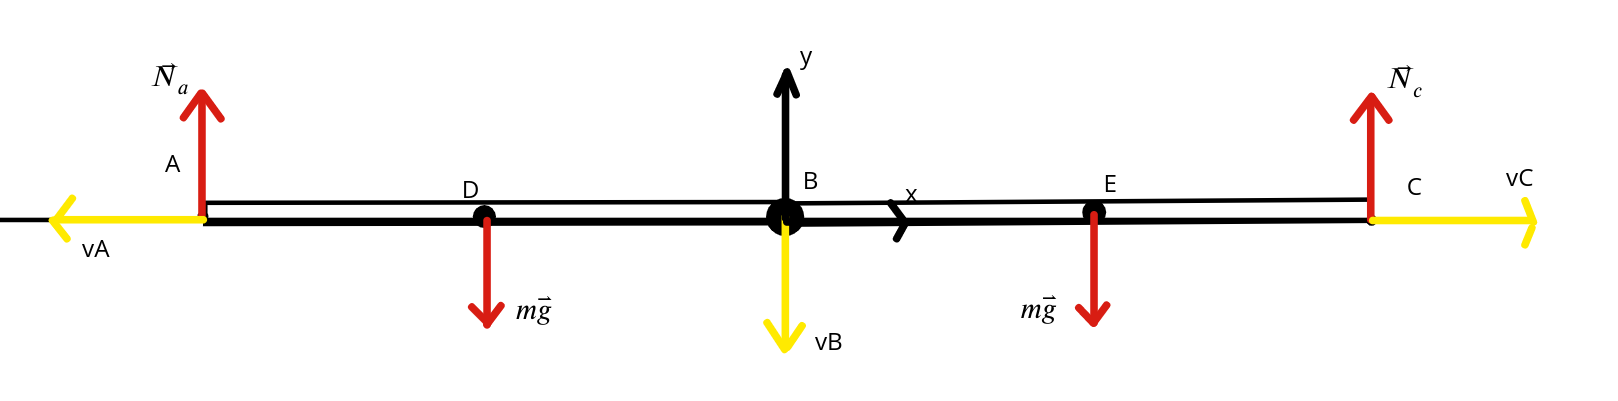
\includegraphics[width=\linewidth]{task2h.png}
          \begin{tabular}{|c|c|c|}
              \hline
              $$    & $initial$            & $final$                  \\
              \hline
              $x_b$ & $0$                  & $0$                      \\
              \hline
              $y_b$ & $h$                  & $0$                      \\
              \hline
              $x_c$ & $\sqrt{4l^2 - h^2}$  & $\sqrt{4l^2 - h^2} + h$  \\
              \hline
              $y_c$ & $0$                  & $0$                      \\
              \hline
              $x_a$ & $-\sqrt{4l^2 - h^2}$ & $-\sqrt{4l^2 - h^2} - h$ \\
              \hline
              $y_a$ & $0$                  & $0$                      \\
              \hline
          \end{tabular}
    \item Solution:
          \begin{enumerate}
              \item Kinetic energy:
                    \begin{align}
                        T_{AB} = \frac{1}{2}I\omega_{AB}^2 \\
                        T_{BC} = \frac{1}{2}I\omega_{BC}^2
                    \end{align}
              \item Inertia of the rod: \\
                    I will use Huygens–Steiner theorem to find moment of inertia. \\
                    \begin{align}
                        I = m_{AB}l^2 + m_{AB}\rho^2
                    \end{align}
              \item Angular velocity of the rods: \\
                    IC of velocity for rod $AB$ at the final will be at $A$, $BC$ at $C$. \\
                    \begin{align}
                        v_B = \omega_{AB} \cdot 2l \\
                        v_B = \omega_{BC} \cdot 2l
                    \end{align}
              \item Work done by external forces: \\
                    \begin{align}
                        A_{if} = mg \frac{h}{2} + mg \frac{h}{2}
                    \end{align}
              \item Equation of change:
                    \begin{align}
                        T_{AB} + T_{BC} = A_{if}                                                                                        \\
                        \frac{1}{2}I \cdot (\frac{v_B}{2l})^2 + \frac{1}{2}I \cdot (\frac{v_B}{2l})^2 = mg \frac{h}{2} + mg \frac{h}{2} \\
                        v_B = 2l \sqrt{\frac{gh}{l^2 + \rho^2}}
                    \end{align}
          \end{enumerate}
\end{enumerate}

\subsection*{Task 2 (next part)}

This part is pretty much the same as the previous one, but with a different final conditions.

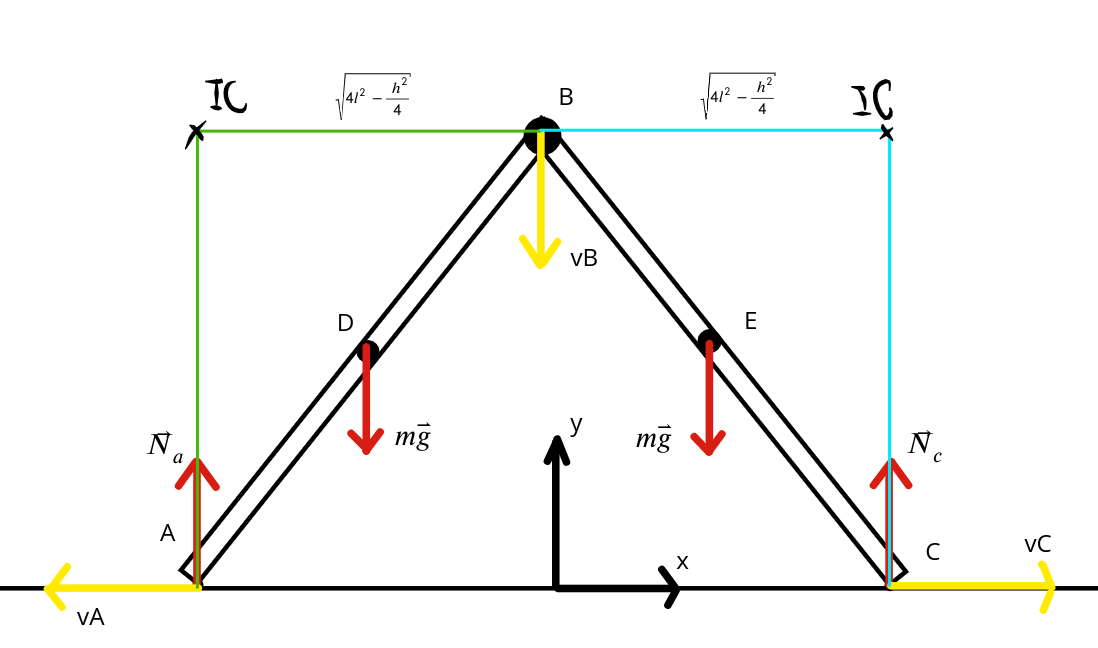
\includegraphics[width=\linewidth]{task2ic.png}

\begin{enumerate}
    \item Conditions: \\
          \begin{tabular}{|c|c|c|}
              \hline
              $$    & $initial$            & $final$                    \\
              \hline
              $x_b$ & $0$                  & $0$                        \\
              \hline
              $y_b$ & $h$                  & $h/2$                      \\
              \hline
              $x_c$ & $\sqrt{4l^2 - h^2}$  & $\sqrt{4l^2 - h^2} + h/2$  \\
              \hline
              $y_c$ & $0$                  & $0$                        \\
              \hline
              $x_a$ & $-\sqrt{4l^2 - h^2}$ & $-\sqrt{4l^2 - h^2} - h/2$ \\
              \hline
              $y_a$ & $0$                  & $0$                        \\
              \hline
          \end{tabular}
    \item Angular velocities of the rods: \\
          IC is shown on picture above: \\
          \begin{align}
              v_B = \omega_{AB} \cdot \sqrt{4l^2 - \frac{h^2}{4}} \\
              v_B = \omega_{BC} \cdot \sqrt{4l^2 - \frac{h^2}{4}}
          \end{align}
    \item Work done by external forces: \\
          \begin{align}
              A_{if} = mg \frac{h}{4} + mg \frac{h}{4}
          \end{align}
    \item Equation of change:
          \begin{align}
              T_{AB} + T_{BC} = A_{if}                                                                                                                                                  \\
              \frac{1}{2}I \cdot \big(\frac{v_B}{\sqrt{4l^2 - \frac{h^2}{4}}}\big)^2 + \frac{1}{2}I \cdot (\frac{v_B}{\sqrt{4l^2 - \frac{h^2}{4}}})^2 = mg \frac{h}{4} + mg \frac{h}{4} \\
              v_B = \frac{1}{2} \sqrt{16l^2 - h^2} \sqrt{\frac{gh}{2 (l^2 + \rho^2) }}
          \end{align}
\end{enumerate}

\subsubsection*{Answer:}

\begin{answer}
    \begin{enumerate}
        \item \begin{align}
                  v_B = 2l \sqrt{\frac{gh}{l^2 + \rho^2}} \notag
              \end{align}
        \item \begin{align}
                  v_B = \frac{1}{2} \sqrt{16l^2 - h^2} \sqrt{\frac{gh}{2 (l^2 + \rho^2) }} \notag
              \end{align}
    \end{enumerate}
\end{answer}

